%%%%%%%%%%%%%%%%%%%%%%%%%%%%%%%%%%%%%%%%%%%%%%%
% LATEX UT THESIS TEMPLATE 							      	   	 %
% By Elahe Rannai									        	 %
% No rights reserved. The author appreciates any distribution and/or completion of this material.  	 %
%%%%%%%%%%%%%%%%%%%%%%%%%%%%%%%%%%%%%%%%%%%%%%%
\documentclass[twoside, a4paper,11pt]{book}
\usepackage[margin=10mm,font={footnotesize},labelfont={footnotesize}]{caption}

\usepackage{amsmath}
\usepackage{graphicx}
\usepackage[multidot]{grffile}
\usepackage{wrapfig}
\usepackage{verbatim}
\usepackage{fancyhdr}
\usepackage{url}
\usepackage{hyperref}
\usepackage{supertabular}
\usepackage{multicol}
\usepackage{setspace}
\usepackage{changepage}
\usepackage{color}
\usepackage{array}
\usepackage{colortbl}

\usepackage{amsmath}
\usepackage{amsthm}
\usepackage{amssymb}
\usepackage{cancel}
\usepackage{mathtools}
\usepackage{extpfeil}

\usepackage{subfigure}
\usepackage{tabularx}
\usepackage{multirow}
\usepackage{afterpage}


\usepackage{cite}
%\usepackage{cleveref}
\usepackage[rgb,x11names]{xcolor}% Optimize for screen reading.


\usepackage{algorithm}
\usepackage{algorithmic}
\usepackage[xindy]{glossaries}

\usepackage{zref-abspage}
\usepackage{perpage}
\MakePerPage{footnote}

\usepackage{hhline}
\usepackage[T1]{fontenc}
\usepackage{xcolor}    % loads also »colortbl«

\definecolor{stBlue}{RGB}{0,176,240}
\definecolor{stGreen}{RGB}{0,204,0}
\definecolor{stRed}{RGB}{255,0,0}
\definecolor{stYellow}{RGB}{255,255,0}
\definecolor{stOrange}{RGB}{255,192,0}
\definecolor{stPink}{RGB}{255,153,153}
\definecolor{stGray}{RGB}{191,191,191}
\definecolor{stPurple}{RGB}{112,48,160}
\definecolor{stBrown}{RGB}{204,153,0}
\definecolor{stLightGreen}{RGB}{153,255,153}
\definecolor{stLightPurple}{RGB}{204,153,255}



\usepackage[extrafootnotefeatures]{xepersian}
\LTRcolumnfootnotes


\numberwithin{equation}{chapter}
\numberwithin{table}{chapter}
\numberwithin{figure}{chapter}
\numberwithin{equation}{chapter}


\settextfont[Scale=1.12]{XB Niloofar}
\setlatintextfont[Scale=1.05]{Times New Roman}

\DefaultMathsDigits
\DeclareMathSizes{10}{12}{8}{6}   % For size 10 text


\defpersianfont\nastaliq[Scale=1]{IranNastaliq}
\defpersianfont\nastaliqbig[Scale=1.3]{IranNastaliq}


\linespread{2.04}
\setlength\parskip{0.25cm}
\setlength\topmargin{-0.5in}
\setlength\headheight{2cm}
\setlength\headsep{0.7cm}
\setlength\textheight{8.997in}
\setlength\textwidth{5.9078in}
\setlength\oddsidemargin{-0.0158in}
\setlength\evensidemargin{0.38in}

\setlength{\parindent}{1cm}

\newenvironment{strict_enumerate}
{\begin{enumerate}
  \setlength{\itemsep}{0.1pt}
  \setlength{\parskip}{0pt}
  \setlength{\parsep}{0pt}}
{\end{enumerate}}

\newenvironment{strict_itemize}
{\begin{itemize}
  \setlength{\itemsep}{1pt}
  \setlength{\parskip}{0pt}
  \setlength{\parsep}{0pt}}
{\end{itemize}}


\newenvironment{strict_description}
{\begin{description}
  \setlength{\itemsep}{1pt}
  \setlength{\parskip}{0pt}
  \setlength{\parsep}{0pt}}
{\end{description}}


\newglossarystyle{mylistFa}{
\glossarystyle{list}
\renewenvironment{theglossary}{}{}
\renewcommand*{\glossaryheader}{}
\renewcommand*{\glsgroupheading}[1]{}
\renewcommand*{\glsgroupskip}{}
\renewcommand*{\glossaryentryfield}[5]     {\noindent\glstarget{##1}{##2}\dotfill \space \lr{##3} \\}
\renewcommand*{\glossarysubentryfield}[6]{\glossaryentryfield{##2}{##3}{##4}{##5}{##6}}
}

\newglossarystyle{mylistLa}{
\glossarystyle{list}
\renewenvironment{theglossary}{}{}
\renewcommand*{\glossaryheader}{}
\renewcommand*{\glsgroupheading}[1]{}
\renewcommand*{\glsgroupskip}{}
\renewcommand*{\glossaryentryfield}[5]     {\noindent\glstarget{##1}{##3}\dotfill \space ##2 \\}
\renewcommand*{\glossarysubentryfield}[6]{\glossaryentryfield{##2}{##3}{##4}{##5}{##6}}
}

\newglossary[glg]{latin}{gls}{glo}{واژه‌نامه‌ انگلیسی به فارسی}
\newglossary[blg]{persian}{bls}{blo}{واژه‌نامه‌ فارسی به انگلیسی}

\newcommand{\mls}[1]{\gls{fa-#1}\glsuseri{la-#1}}

\newcommand{\inpdic}[2]{
	\newglossaryentry{fa-#1}{type=persian,name={#1}, sort={#1},description={#2}}
	\newglossaryentry{la-#1}{type=latin,name=\lr{#2}, sort={#2},description={#1}}
}


\makeatletter
\renewcommand*{\cleardoublepage}{\clearpage\if@twoside \ifodd\c@page\else
\hbox{}%
\thispagestyle{empty}%
\newpage%
\if@twocolumn\hbox{}\newpage\fi\fi\fi}

%meee error ! LaTeX Error: \gls@persian@displayfirst undefined.
%\renewcommand{\gls@persian@displayfirst}[4]{
	%#1#4\protect\LTRfootnote{#2}
%}
\defglsdisplayfirst[persian]{#1#4\protect\LTRfootnote{#2}}

%\makeatother
\makeglossaries
\glsdisablehyper
\inpdic{بازی‌های شناختی}{Cognitive Games}
\inpdic{توانایی‌های شناختی}{Cognitive Abilities}
\inpdic{تمرین‌های شناختی}{Cognitive training}
\inpdic{توجه و تمرکز}{Attention}
\inpdic{توجه}{Attention}
\inpdic{حافظه}{Memory}
\inpdic{حل مساله}{Problem Solving}
\inpdic{استراتژی}{Strategy}
\inpdic{استراتژی یادگیری}{Learning Strategy}
\inpdic{راهبرد}{Strategy}
\inpdic{راهبرد یادگیری}{Learning Strategy}
\inpdic{تکرار کردن}{Rehearsal}
\inpdic{برقرار کردن ارتباط معنایی}{Semantic}
\inpdic{گروه کردن}{Grouping}
\inpdic{تماس چشمی}{Eye contact}
\inpdic{توضیح دادن}{Paraphrasing}
\inpdic{گفتگو با خود}{self-talk}
\inpdic{توجه تقسیم شده}{Divided Attention}
\inpdic{ردیابی همزمان چندین شیء}{Multiple Object Tracking}
\inpdic{ادراک}{Perception}
\inpdic{مهارت‌های حرکتی}{Motor Skills}
\inpdic{کارکردهای اجرایی}{Executive Functions}
\inpdic{بیش‌فعالی}{ADHD}
\inpdic{اختلال کمبود توجه}{ADD}
\inpdic{فعالیت‌ها}{task}
\inpdic{شرکت‌کننده}{subject}
\inpdic{حافظه‌ی کاری}{Working Memory}
\inpdic{هوش سیال}{Fluid Intelligence}
\inpdic{انجام چند کار همزمان}{Multitasking}
\inpdic{ظرفیت حافظه‌ی کاری}{Working Memory Capacity}
\inpdic{هوش متبلور}{Crystallized Intelligence}
\inpdic{انگیزه}{Motivation}
\inpdic{انتقال}{transfer}
\inpdic{مقاومت در برابر چالش}{Persistence}
\inpdic{تجسم فضایی}{Spatial Skills}
\inpdic{آموزش استراتژی}{Strategy training}
\inpdic{آموزش راهبرد}{Strategy training}
\inpdic{حافظه‌ی کاری کلامی}{Verbal working memory}
\inpdic{درک مطلب شنیداری}{Passage listening comprehension}
\inpdic{منحرف کننده}{distractor}
\inpdic{حرکات چشم}{saccade}
\inpdic{مبتنی بر مدل}{model-based}
\inpdic{غیر مبتنی بر مدل}{model-free}
\inpdic{آزمون دو مرحله‌ای دا}{daw two step task}
\inpdic{قدم زدن تصادفی}{random walk}
\inpdic{بدنه‌ی محدب}{convex hull}
\inpdic{دمای معکوس}{inverse temperature}
\inpdic{نمودار احتمال نرمال بودن}{normal probability plot}
\inpdic{داده‌های پرت}{outliers}
\inpdic{یادگیری ماشین}{machine learning}
\inpdic{یادگیری تقویتی}{reinforcement learning}
\inpdic{میانه انحراف مطلق}{median absolute deviation}
\inpdic{پیرسون}{Pearson}
\inpdic{نمودار نقطه‌ای}{scatter plot}
\inpdic{ویلکاکسون}{Wilcoxon}
\inpdic{کروسکال-والیس}{Kruskal-Wallis}
\inpdic{هیستوگرام}{Histogram}
\inpdic{تیم مغزینه}{maghzineh.com}
\inpdic{توجه پایدار}{Sustained Attention}
\inpdic{توجه انتخابی}{Selective Attention}
\inpdic{توجه متناوب}{Alternating Attention}
\inpdic{توجه تقسیم‌شده}{Divided Attention}
\inpdic{برخط}{online}
\inpdic{منحرف‌کننده}{distractor}
\inpdic{آنالیز واریانس}{ANOVA}
\inpdic{کولموگروف-اسمیرنف}{Kolmogorov–Smirnov}
\inpdic{پیشین}{pre-test}
\inpdic{پسین}{post-test}



\begin{document}
% Besmellah Page
\newpage
\thispagestyle{empty}
\begin{center}
\begin{tabular}{c}
\\ \\ \\ \\ \\

\includegraphics[scale=0.7, origin=c]{Figures/besm1.jpg}\\
\end{tabular}
\end{center}
%


\newpage
\thispagestyle{empty}
\mbox{}

%%%%%%%%%%%%%%%%%
%TITLE PAGE
%%%%%%%%%%%%%%%%%
\newpage
\thispagestyle{empty}
\begin{center}
\begin{tabular}{lp{7cm}r}

\includegraphics[width=2.8cm]{Figures/ut.png} & & 
\includegraphics[width=3.8cm]{Figures/eng.png} \\
\end{tabular}

{\LARGE\bfseries دانشگاه \space تهران}
\\*
{\Large\bfseries پردیس دانشکده‌های فنی}
\\*
{\Large\bfseries دانشکده‌ مهندسی برق و کامپیوتر}
\par
\vskip 1.4cm
{\Huge\bfseries استخراج استراتژی‌های موثر در یک بازی شناختی در حوزه‌ی توجه و تمرکز و بررسی تاثیر آموزش آن بر افراد مبتدی}\par
\vskip .9cm
{\large%
  نگارش }\par
{\Large\bfseries الهه ابوالحسنی شهرضا}\par
\par
{\large
  استاد راهنما\par
\Large\bfseries دکتر مجید نیلی  \\

}
\par
\vskip 1.4cm
{\large\bfseries پایان‌نامه برای دریافت درجه کارشناسی‌ارشد در رشته \\* مهندسی کامپیوتر - گرایش هوش مصنوعی}
\par
\vskip .5cm
{\large شهریور ۱۳۹۶}
\par
\vfill
\end{center}

%%%%%%%%%%%%%%%%%%%%
%\newpage
%\thispagestyle{empty}
%\mbox{}

%\newpage
%\thispagestyle{plain}
%\begin{center}
%\begin{tabular}{lp{7cm}r}
%\includegraphics[width=15cm]{Figures/Table.png} 
%\end{tabular}
%\end{center}
%%%%%%%%%%%%%%%%%%%%%%
\newpage
\thispagestyle{empty}
\mbox{}

\newpage
\thispagestyle{plain}
\begin{center}
\begin{tabular}{lp{7cm}r}

\includegraphics[width=2.8cm]{Figures/ut.png} & & 
\includegraphics[width=3.8cm]{Figures/eng.png} \\
\end{tabular}

{\LARGE\bfseries دانشگاه \space تهران}
\\*
{\Large\bfseries پردیس دانشکده‌های فنی}
\\*
{\Large\bfseries دانشکده مهندسی برق و کامپیوتر}
\par
پایان نامه برای دریافت درجه کارشناسی ارشد در رشته مهندسی کامپیوتر

\vskip 1cm
\par
عنوان:

{\Large\bfseries استخراج استراتژی‌های موثر در یک بازی شناختی در حوزه‌ی توجه و تمرکز و بررسی تاثیر آموزش آن بر افراد مبتدی}

\vskip .2cm
{\Large نگارش: الهه ابوالحسنی شهرضا}
\end{center}
\vskip .3cm

\noindent
این پایان‌نامه در تاریخ ۱۳۹۶/۰۶/۱۲ در مقابل هیأت داوران دفاع گردید و مورد تصویب قرار گرفت.
\vskip .5cm
\begin{tabular}{r r}
معاون آموزشی و تحصیلات تکمیلی پردیس دانشکده‌های فنی: دکتر جلیل آقا راشد محصل \\
رئیس دانشکده مهندسی برق و کامپیوتر: دکتر مجید نیلی\\
معاون پژوهشی و تحصیلات تکمیلی: دکتر بابک نجار اعرابی \\
استاد راهنما: آقای دکتر مجید نیلی \\
استاد راهنمای دوم: آقای دکتر هادی مرادی\\
عضو هیأت داوران: خانم دکتر فتانه تقی‌یاره \\
عضو هیأت داوران: آقای دکتر بهروز مینایی \\

\end{tabular}



\newpage
\thispagestyle{empty}
\mbox{}

\newpage
\thispagestyle{empty}
{ \LARGE 
\begin{center}
تعهدنامه اصالت اثر
\end{center}}
اینجانب الهه ابوالحسنی شهرضا تایید می‌کنم که مطالب مندرج در این پایان نامه حاصل کار و پژوهش اینجانب بوده و به دستارود‌های پژوهشی دیگران که در این نوشته از آنها استفاده شده است مطابق مقررات ارجاع گردیده است. به‌علاوه این پایان نامه قبلا برای احراز هیچ مدرک هم سطح یا بالاتر ارائه نشده است.
\par
کلیه حقوق مادی و معنوی این اثر متعلق به دانشکده فنی دانشگاه تهران است.
\par 
\vskip 2cm


\begin{flushleft}
نام و نام خانوادگی دانشجو: الهه ابوالحسنی شهرضا \hspace{1.75cm}~~~~~~~ \\
امضای دانشجو: ~~~~~~~~~~~~~~~~~~~~~~~~~~~~~~~~~~~~~~~~~~~~~~~~~~~~~
\end{flushleft}

\newpage
\thispagestyle{empty}
\mbox{}


%\newpage
%\thispagestyle{empty}
%\mbox{}
%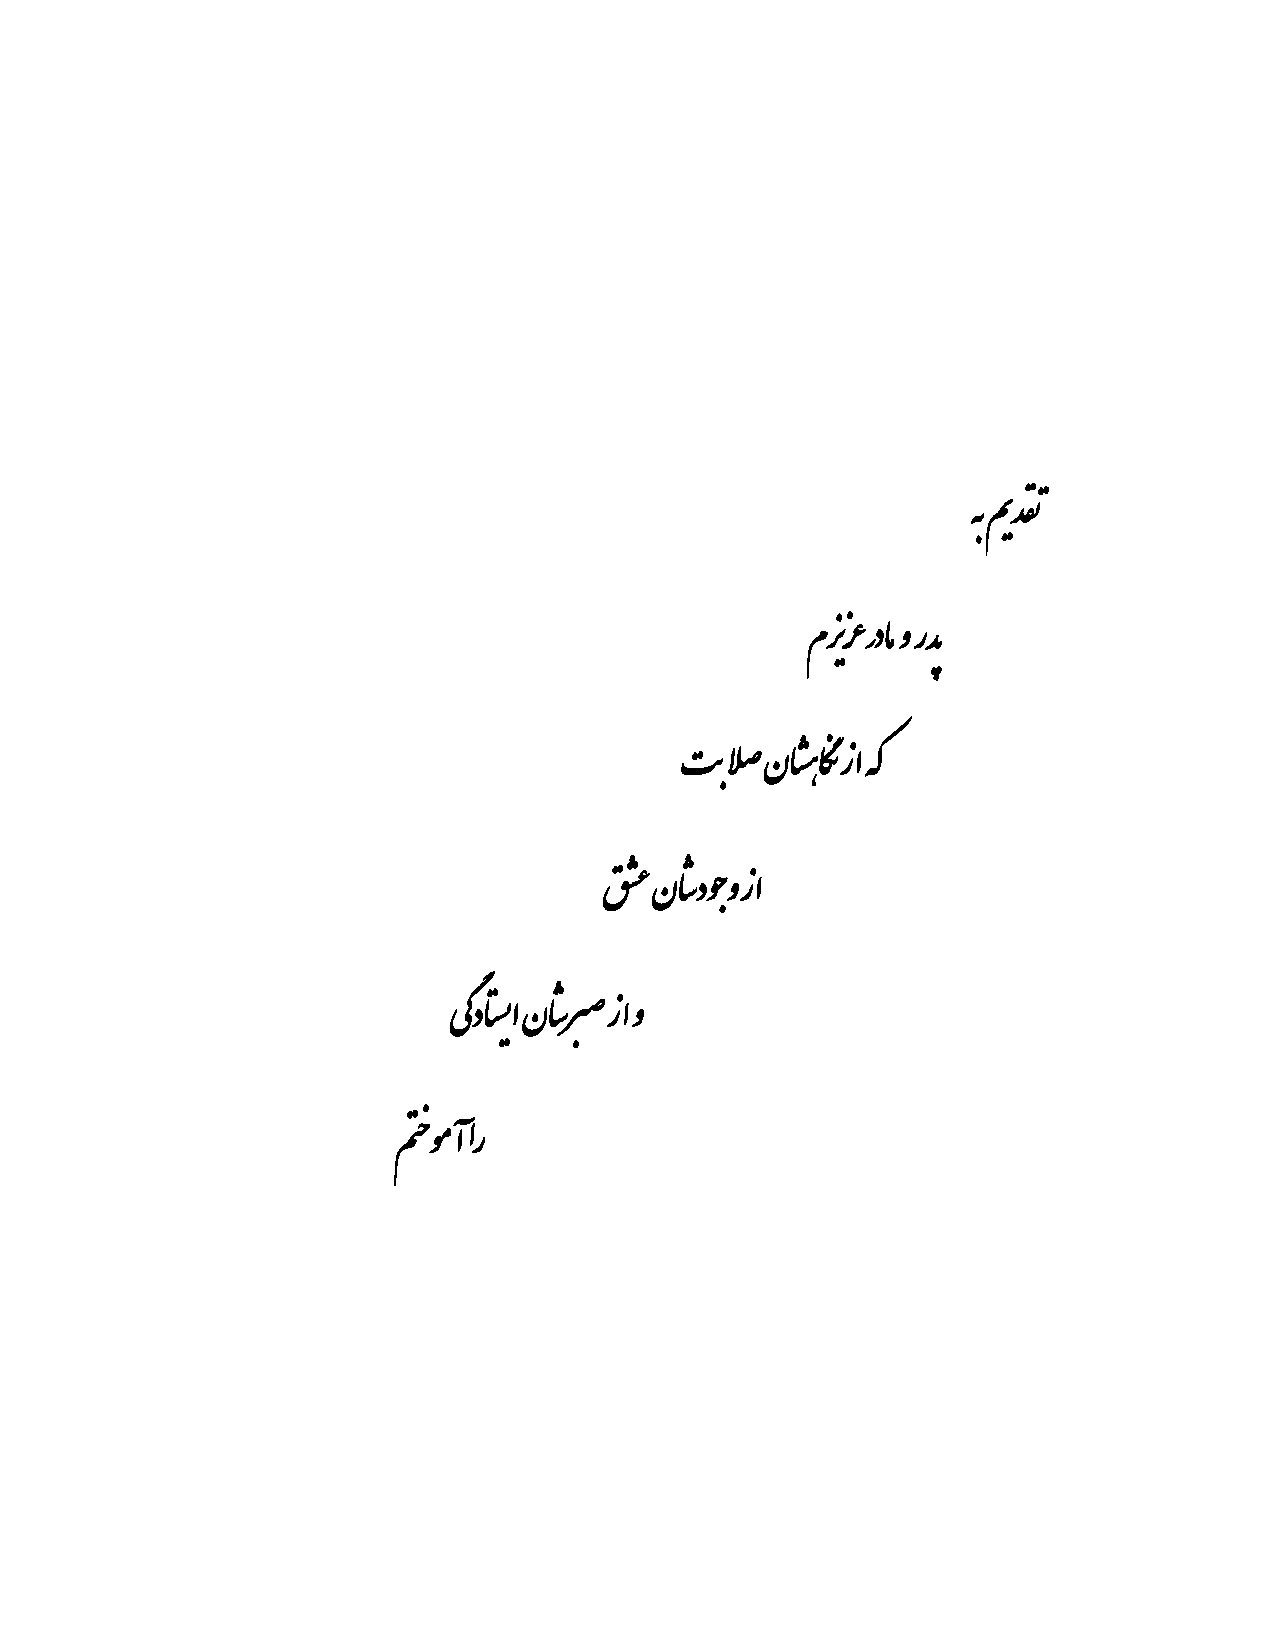
\includegraphics[scale=0.9]{Figures/taghdir.pdf} 


\newpage
\thispagestyle{empty}
\mbox{}


\newpage
\thispagestyle{empty}
{\nastaliqbig \Huge 
تقدیر و تشکر\nastaliq

{\par\vspace{1cm}}
\LARGE
\begin{adjustwidth}{1cm}{}
مراتب تشکر و قدردانی خود را نسبت به تمام کسانی که مرا در انجام این پایان‌نامه یاری کرده‌اند، خصوصاً اساتید گرامی و ارجمندم، جناب آقای دکتر نیلی و جناب آقای دکتر مرادی که رهنمودهای ایشان همواره راهگشای پیچیدگی‌های این پژوهش بوده است، ابراز می‌دارم. 

همچنین، از تمامی دوستانم در آزمایشگاه رباتیک شناختی که با حضور و محبتشان مرا یاری نمودند تشکر و قدردانی می‌نمایم. 

\end{adjustwidth}
}


\newpage
\thispagestyle{empty}
\mbox{}


\pagestyle{plain}

\newpage

\begin{center}
\vspace*{-2.6cm}
\subsection*{چکیده}
\end{center}
\vspace*{-.4cm}

\begin{spacing}{1.8}
با توجه به رشد روز‌‌افزون اطلاعات موجود در وب، موتورهای جست‌و‌جو در بازیابی اطلاعات مورد نیاز کاربران از میان حجم زیادی از اطلاعات نقشی اساسی ایفا می‌کنند. با بررسی رفتار کاربر در اینترنت مشاهده شده است که بیشترین بازدید از یک صفحه وب، به واسطه نتایج اولیه بازیابی شده توسط موتورهای جست‌و‌جو می‌باشد. با توجه به این امر، ایده هرزنویسی در وب با هدف افزایش رتبه صفحات هرز در میان نتایج موتورهای جست‌و‌جو مطرح شد. برای شناسایی و مقابله با این صفحات روش‌هایی ارائه شده است که می‌توان آن‌ها را به سه دسته کلی روش‌های مبتنی بر محتوا، روش‌های مبتنی بر پیوند و روش‌های مبتنی بر داده‌های جانبی تقسیم نمود. در این پژوهش تمرکز بر روی دو روش اصلی مبتنی بر محتوا و مبتنی بر پیوند و همچنین ترکیب این دو روش به منظور شناسایی وب‌گاه‌های هرز می‌باشد.

از آن‌جایی که عملکرد موتورهای جست‌و‌جو در شناسایی وب‌گاه‌های هرز فارسی پایین می‌باشد، در این پژوهش پس از ساخت یک مجموعه داد‌ه‌ای مناسب شامل وب‌گاه‌های هرز و معتبر فارسی، به بررسی و تحلیل تعدادی از ویژگی‌های محتوایی برای شناسایی وب‌گاه‌های هرز فارسی می‌پردازیم. سپس با ارائه چندین ویژگی محتوایی جدید و استفاده از روش‌های انتخاب ویژگی، کارایی رده‌بندی وب‌گاه‌ها را افزایش می‌دهیم. در ادامه، یک سامانه جدید شناساگر هرز وب فارسی را ارائه می‌دهیم که از مدل بهبود یافته کیف کلمات برای استخراج ویژگی‌ها استفاده می نماید و نسبت به روش‌های محتوایی پیشین کارایی بالاتری دارد. با توجه به گسترش استفاده از الگوریتم‌های مبتنی بر پیوند در روش‌های هرزنویسی، تعدادی از الگوریتم‌های مهم در این زمینه را مورد بررسی قرار داده و دو الگوریتم جدید ارائه می‌دهیم که بسیاری از نقاط ضعف الگوریتم‌های پیشین را ندارند. در الگوریتم اول برای بهبود انتشار امتیاز اعتماد در گراف وب، از سه سیاست انتخاب بهینه گره‌های بذر، وزن‌دهی به یال‌های گراف برای مشخص کردن میزان اعتبار یال‌ها، و بسط دوره‌ای گره‌های بذر استفاده می‌شود. در الگوریتم دوم با استفاده از انتشار امتیاز هرز، هم‌زمان به صورت پیش‌رو و پس‌رو در سراسر گراف وب، کیفیت رتبه‌بندی وب‌گاه‌های هرز را بهبود می‌دهیم.
در آخر نیز به منظور بهبود کیفیت رتبه‌بندی وب‌گاه‌ها روشی پیشنهاد داده می‌شود که برای انتشار امتیاز وب‌گاه‌ها، از احتمال اعتبار و هرز بودن محتوایی وب‌گاه‌ها در تمام بخش‌های گراف استفاده می‌نماید. 

در پایان این پژوهش، به منظور ارزیابی روش‌ها و بررسی میزان کارایی آن‌ها، آزمایش‌های مربوطه انجام شده است. نتایج آزمایش‌ها نشان می‌دهد که روش‌های ارائه شده در مقایسه با روش‌های قبلی، از کارایی و دقت بالاتری برخوردار هستند.
 
\textbf{واژه‌های کلیدی: }\textit{هرزنویسی، هرز وب، شناسایی هرز، انتشار برچسب، ویژگی‌های محتوایی.}
\end{spacing}

\pagenumbering{harfi}


\newpage
\thispagestyle{empty}
\mbox{}

\renewcommand\listfigurename{فهرست شکل‌ها}
\renewcommand\listtablename{فهرست جدول‌ها}
%\renewcommand{\refname}{مراجع}

\begin{doublespace}\small{
\tableofcontents
\listoftables
\listoffigures
}\end{doublespace}





\pagestyle{fancy}	
\fancyhead{} 
\fancyhead[RO]{\leftmark}
\fancyhead[LO]{\thepage}
\fancyhead[LE]{\rightmark}
\fancyhead[RE]{\thepage}
\fancyfoot{} 
\renewcommand{\headrulewidth}{0.6pt} 
\renewcommand{\footrulewidth}{0pt}

\chapter{مقدمه}
\label{chapter:introduction}
\pagenumbering{arabic}\setcounter{page}{1}
\thispagestyle{plain}

طبق تعریف \mls{بازی‌های شناختی} بازی‌هایی هستند که هدف آنها بهبود \mls{توانمندی‌های شناختی} بازیکنان است. در این بازی‌ها سعی می‌شود توانمندی‌های شناختی مانند \mls{توجه و تمرکز}، \mls{حافظه}  و \mls{حل مساله}  بهبود پیدا کنند. این بازی‌ها به منظور استفاده‌ی عموم مردم طراحی شده‌اند. با وجود توسعه و استفاده‌ی روز افزون از این بازی‌ها نتایج برخی از تحقیقات انجام شده (\cite{melby2013WM}، \cite{redick2013Intellig}) نشان می‌دهند در بسیاری از موارد تاثیرگذاری مورد انتظار را نداشته‌اند.\\
هدف نهایی بازی‌های شناختی بهبود توانمندی‌های شناختی افراد است. بهبود این توانمندی‌ها در هر فرد باعث بهبود کیفیت زندگی او می‌شود و آسیب‌های شناختی احتمالی ناشی از کهولت سن یا حوادث را به تعویق می‌اندازد. در اصل این بازی‌ها نوعی ورزش مغزی محسوب می‌شوند.\\
پرسشی که ایجاد می‌شود این است که آیا می‌توان با تغییر دادن بازی‌های شناختی و شخصی سازی آنها به بهبود تاثیرگذاری این بازی‌ها کمک کرد؟ آیا می‌توان با توجه به نقاط ضعف و قوت بازیکن به نحوی بازی را تغییر داد که بیشترین تاثیرگذاری ممکن اتفاق بیافتد؟\\
یکی از روش‌های رایج به منظور بهبود عملکرد افراد در حوزه‌های مختلف، مانند توانبخشی شناختی []، آموزش زبان دوم [] و یا عملکرد دانشگاهی [] آموزش \mls{استراتژی} است. منظور از استراتژی در این پژوهش، \mls{استراتژی یادگیری}  است. استراتژی یادگیری به فرآیندهایی گفته می‌شود که وقتی با نیازمندی‌های یک تمرین مطابقت پیدا می‌کنند باعث بهبود عملکرد می‌شوند \cite{donker2014LearningSt}.\\
استراتژی‌های مربوط به بهبود حافظه شناخته‌شده‌تر هستند. به عنوان مثال می‌توان به استراتژي \mls{تکرار کردن} ، \mls{برقرار کردن ارتباط معنایی}  یا \mls{گروه کردن}  اشاره کرد \cite{morrison2016WM}. اما روی استراتژی‌های مربوط به بهبود توجه کمتر کار شده است. از استراتژی‌های شناخته شده در حوزه‌ی توجه می‌توان به \mls{تماس چشمی} ، \mls{توضیح دادن}  یا \mls{گفتگو با خود} اشاره کرد \cite{twamley2008CogTrain}.\\
در این پژوهش هدف نهایی طراحی یک بازی شناختی تطبیق‌پذیر با بازیکن است که می‌تواند با توجه به نحوه‌ی عملکرد او روش بازی‌اش را استخراج کند و سپس استراتژی‌هایی را به او آموزش دهد که باعث بهبود عملکرد وی در بازی و نهایتا در زندگی واقعی می‌شود.\\
استراتژی‌های مربوط به توجه تا به امروز مورد توجه قرار نگرفته بودند و استراتژی‌های بسیار محدودی برای آن مطرح شده بود. در این پژوهش سعی شده است مجموعه‌ای از استراتژی‌های مربوط به «\mls{توجه تقسیم شده}» معرفی شوند.\\
علاوه بر این، این پژوهش یک چارچوب جهت استفاده از آموزش استراتژی در بازی‌های مختلف ارائه می‌دهد که می‌توان از آن برای بازی‌های دیگر نیز استفاده کرد.\\
به منظور دستیابی به اهداف این پژوهش یک بازی شناختی با نام «ابر باران‌زا» انتخاب شد که هدف اصلی آن بهبود شاخه‌ی «توجه تقسیم‌شده» از زیرشاخه‌های «توجه» است.\\
این پژوهش شامل دو فاز عمده است. فاز اول را فاز استخراج استراتژی و فاز دوم را فاز انتقال استراتژی می‌نامیم.\\
در فاز اول دو هدف پیگیری می‌شوند. هدف اول گردآوری استراتژی‌هایی است که افراد در این بازی استفاده می‌کنند و هدف دوم بررسی میزان اثرگذاری این استراتژی‌ها است. به این معنا که هر کدام از این استراتژی‌ها به صورت میانگین چقدر توانسته‌اند برای این بازیکن امتیاز به دست بیاورند.\\
در فاز دوم هدف بررسی تاثیر انتقال این استراتژی‌ها به افرادی است که عملکرد ضعیف‌تری داشته‌اند. (تکمیل شود)\\







%%%%%%%%%%%%%%%%%%%%%%%%%%%%%%%%%%%%%%%%%%%%%%%%%%%%%%
%\newpage
%\thispagestyle{empty}
%\mbox{}

\chapter{پژوهش‌های پیشین}
\label{chapter:relatedWork}
\thispagestyle{plain}
در این فصل، پژوهش‌های پیشین را سه بخش ارائه می‌دهیم: بازی‌های شناختی، استفاده از آموزش استراتژی در بازی‌ها، پژوهش‌های انجام شده روی فعالیت \mls{ردیابی همزمان چندین شیء}\\
\section{بازی‌ها و تمرین‌های شناختی}
بازی‌های شناختی بازی‌هایی هستند که تلاش می‌کنند توانمندی‌های شناختی افراد را تقویت کنند. توانمندی‌های شناختی مهارت‌های ذهنی هستند که برای انجام دادن ساده‌ترین تا پیچیده‌ترین کارها مورد نیاز هستند. این مهارت‌ها شامل \mls{ادراک}، \mls{توجه} ، \mls{حافظه} ، \mls{مهارت‌های حرکتی} و\mls{کارکردهای اجرایی} هستند.
یکی از مهم‌ترین مسائلی که در رابطه با بازی‌های شناختی مطرح می‌شود مساله‌ی میزان تاثیرگذاری این بازی‌ها است. سوالاتی که در این زمینه مطرح می‌شوند از این دست هستند: آیا بازی کردن با یک بازی مخصوص حافظه باعث می‌شود حافظه‌ی فرد بازیکن بهبود پیدا کند؟ چه مدت باید این بازی صورت بگیرد؟ بازیکن باید چه شرایطی داشته باشد؟ مدت‌زمان تاثیرگذاری بازی چه مدت است؟

یکی دیگر از سوالاتی که مطرح می‌شود این است که آیا تمرین کردن یک تمرین که روی یک توانایی شناختی تمرکز دارد باعث بهبود سایر توانمندی‌های شناختی نیز می‌شود؟ به این پدیده به اصطلاح \mls{انتقال} گفته می‌شود. به عنوان مثال آیا انجام دادن تمرین در حوزه‌ی \mls{حافظه‌ی کاری} باعث بهبود \mls{هوش سیال} هوش سیال می‌شود؟

در سال ۲۰۱۱ جائگی  \cite{jaeggi2011shortLong} تاثیرگذاری طولانی مدت و کوتاه مدت تمرین‌های شناختی را بررسی کرد. همچنین در تاثیرگذاری تمرین در یک حوزه‌ی شناختی بر بهبود عملکرد در یک حوزه‌ی شناختی دیگر بررسی شده است و نتیجه گرفته شده است که این دو حوزه بر یکدیگر اثرگذار هستند. به این نوع اثرگذاری در ادبیات این پژوهش انتقال  گفته می‌شود. در  \cite{jaeggi2011shortLong} انجام دادن تمرین‌هایی مرتبط با حوزه‌ی حافظه‌ی کاری انجام گرفته است و در نهایت عملکرد افراد در تمرین‌های مرتبط با هوش سیال  ارزیابی شده است. نتیجه‌ی نهایی این است که افرادی که تمرین‌های مربوط به حافظه‌ی کاری را انجام داده‌اند در تمرین‌های مربوط به هوش سیال بهتر عمل کرده‌اند و در نتیجه انتقال اتفاق افتاده است. \cite{jaeggi2011shortLong}  همچنین به بررسی تاثیر طولانی (۲ ماه) مدت این انتقال پرداخته است و نتیجه گرفته است که این تاثیرات در طولانی مدت نیز وجود داشته‌اند. 

در سال ۲۰۱۳ ملبی لرواگ \cite{melby2013WM} در یک پژوهش جامع مقالات متعددی را که تاثیرگذاری تمرین‌های شناختی در حوزه‌ی  \mls{حافظه‌ی کاری} را بررسی کرده بودند ارزیابی کرد. در این مقاله ابتدا معیارهایی برای سنجش یک پژوهش صحیح در این حوزه معرفی شده‌اند و سپس پژوهش‌های متعددی از نظر تاثیرگذاری ارزیابی شده‌اند. ملبی لرواگ در این پژوهش معتقد است یکی از دلایل تشتت آرا در زمینه‌ی تاثیرگذاری تمرین‌های شناختی استاندارد نبودن پژوهش‌ها و روش‌هایی است که در آنها استفاده شده است. نهایتا با توجه به معیارهای معرفی شده ۲۳ مطالعه‌ی انجام شده بررسی شده‌اند. در نهایت نتیجه‌ای که از این پژوهش گرفته شده است این است که تمرینات شناختی در حوزه‌ی حافظه‌ی کاری باعث می‌شوند فرد در کوتاه مدت و در تمرینات مشابه در همان زمینه عملکرد بهتری داشته باشد اما شواهد کافی برای برای اثبات تاثیرگذاری بر سایر حوزه‌ها وجود ندارد.

همچنین ردیک \cite{redick2013Intellig} در سال ۲۰۱۳ در یک پژوهش تاثیر تمرین‌های مرتبط با حافظه‌ی کاری را روی چندین حوزه‌ی مختلف، مانند \mls{هوش سیال}، \mls{انجام چند کار همزمان}، \mls{ظرفیت حافظه‌ی کاری} و \mls{هوش متبلور} بررسی کرد. در این این پژوهش گروهی از نوجوانان طی ۲۰ جلسه تمریناتی را انجام دادند. آنها قبل از شروع دوره، در میانه‌ی آن و پس از اتمام آن آزمون‌هایی را انجام دادند تا روند پیشرفتشان بررسی شود. علاوه بر افراد اصلی دو گروه کنترلی نیز در مطالعه شرکت داشتند. یک گروه یک تمرین جانبی را در این مدت انجام می‌دادند و گروه دیگر هیچ تمرینی را انجام ندادند. نتایج نشان می‌دهد با وجود اینکه افراد در تمرین‌های انجام شده پیشرفت خوبی داشتند ولی در سایر حوزه‌های شناختی هیچ بهبودی نداشتند.

در سال ۲۰۱۴ جائگی نقش تفاوت‌های فردی را در تاثیرپذیری از تمرین‌های شناختی و میزان انتقال بررسی کرد \cite{jaeggi2013IndiDiff}. ادعایی که مطرح می‌کند این است که دلیل متغیر بودن نتایج مربوط به تحقیقات حوزه‌ی تمرین‌های شناختی می‌تواند تفاوت‌های فردی بین شرکت‌کنندگان باشد که در نظر گرفته نشده است. در این پژوهش جائگی نقش \mls{انگیزه} را به عنوان یک تفاوت فردی بررسی می‌کند. به همین منظور و برای اینکه انگیزه‌ی غیر واقعی ایجاد نکنند از پرداخت پول به شرکت‌کنندگان آزمون خودداری کردند. دو معیار ارزیابی برای انگیزه در نظر گرفته شده است. اولین معیار در رابطه با میزان لذتی است که فرد به علت سختی آزمون تجربه می‌کند و دومین معیار درباره‌ی باور فرد درمورد هوش است. تفاوت بین افرادی که هوش را ثابت می‌پندارند و باور به تغییرپذیری آن ندارند و افرادی که باور دارند هوش تغییر پذیر است بررسی شده است. در نهایت نتیجه گرفته شده است باور فرد درباره‌ی هوش روی میزان \mls{انتقال} تاثیرگذار است. علاوه بر این شرکت‌کنندگان در این پژوهش نسبت به سایر پژوهش‌هایی که به آنها پول پرداخت شده بود از نتایج بهتری برخوردار بودند. اما معیار اول تاثیری روی نتایج شرکت‌کنندگان و میزان انتقال نداشت.

\section{استفاده از آموزش استراتژی در بازی‌ها}

\section{پژوهش‌های انجام شده روی فعالیت ردیابی همزمان چند شیء}


%%%%%%%%%%%%%%%%%%%%%%%%%%%%%%%%%%%%%%%%%%%%%%%%%%%%%%
%\newpage
%\thispagestyle{empty}
%\mbox{}
\chapter{روش تحقیق}
\label{chapter:methodology}
\thispagestyle{plain}

\section{مقدمه}
هدف از انجام این پژوهش بررسی تاثیرگذاری آموزش استراتژی بر کارآیی کاربر در یک بازی شناختی در حوزه‌ی توجه و تمرکز است. در حوزه‌های دیگر مانند حافظه کارهای مشابه صورت گرفته است (رفرنس) بنابراین یکی از دلایل انتخاب حوزه‌ی توجه و تمرکز شناخته شده نبودن استراتژی‌های مطرح در این حوزه بود. استراتژی‌های حوزه‌ی حافظه به قدری شناخته شده هستند که بسیاری از ما هنگام امتحانات مدرسه از آنها استفاده کرده‌ایم. یعنی به صورت عمومی افراد جامعه از آنها استفاده می‌کنند. اما در مورد توجه و تمرکز با اینکه تقاضا زیاد است اما استراتژی‌های مرتبط با آن به اندازه‌ی حافظه شناخته شده نیست.\\
علاوه بر این این حوزه به خودی خود از اهمیت بالایی برخوردار است. بسیاری از افراد از نداشتن تمرکز به هنگام انجام کارهای روزمره‌ی خود شکایت دارند. همچنین اختلالات زیادی در حوزه‌ی توجه و تمرکز وجود دارند (مانند \mls{اختلال کمبود توجه} یا \mls{بیش‌فعالی}).\\
شاید در این نقطه بگوییم بسیاری از حوزه‌های شناختی مانند توجه هستند که هم استراتژی‌های آنها ناشناخته است و هم از درجه اهمیت بالایی برخوردار هستند. ویژگی‌ دیگری که حوزه‌ی توجه را از سایر حوزه‌های شناختی متمایز می‌کند این است که \mls{فعالیت‌ها} و بازی‌های متعددی برای توجه و تمرکز طراحی شده و از آنها استفاده می‌شود. به همین دلیل نیازی به طراحی یک بازی جدید و صحت‌سنجی مجدد آن نیست. 
با توجه به مجموع این عوامل حوزه‌ی توجه و تمرکز انتخاب شد.\\

\section{انتخاب بازی}

بازی‌های متعددی در حوزه‌ی توجه و تمرکز توسعه پیدا کرده‌اند. این بازی‌ها روی فاکتورهای مختلف مانند توجه انتخابی، توجه تقسیم‌شده، توجه پایدار و فراخنای توجه کار می‌کنند. بازی انتخاب شده روی فاکتور توجه تقسیم شده کار می‌کند و بر تقویت توانایی انسان برای تمرکز همزمان روی چند عامل تاکید می‌نماید. هرچقدر این نوع از توجه بهتر باشد یک فرد بهتر می‌تواند چندین کار را به صورت همزمان با هم انجام دهد. 
مهم‌ترین معیار انتخاب این بود که بازی استراتژی‌های متنوع داشته باشد. به این معنا که افراد از استراتژي‌ها مختلف برای انجام بازی استفاده کنند. با توجه به این معیار ۴ بازی به عنوان کاندید انتخاب شدند.
\subsection{بازی‌های انتخاب شده}
بازی ابر باران‌زا: این بازی روی توجه تقسیم‌شده کار می‌کند. بازی به این صورت است که تعدادی ابر باران‌زا و تعدادی ابر عادی در صفحه وجود دارند. این ابرها شروع به حرکت می‌کنند و کم کم ابرهای باران‌زا تبدیل به ابرهای عادی می‌شوند. در نهایت وقتی ابرها از حرکت ایستادند کاربر باید ابرهایی را که در ابتدا باران‌زا بودند مشخص کند.
بازی سنگ-کاغذ-قیچی: این بازی روی ... کار می‌کند. این بازی مشابه بازی سنگ-کاغذ-قیچی مرسوم است با این تفاوت که کاربر با کامپیوتر بازی می‌کند و کامپیوتر برای بازی کردن الگوی مشخصی دارد. کاربر باید الگوی کامپیوتر را بفهمد و سپس با توجه به الگو به نحوی بازی کند که بیشترین امتیاز را به دست بیاورد.
بازی مسافرخانه زنبوری: این بازی روی .... کار می‌کند. بازی به این صورت است که در ابتدا تعدادی کندوی زنبور عسل نمایش داده می‌شود که همه خالی هستند. سپس زنبورها در کندوها رفت و آمد می‌کنند. این رفت و آمد شامل سه حرکت است: از بیرون به داخل کندو می‌روند، از کندو خارج می‌شوند یا بین کندوها جابجا می‌شوند. پس از اینکه حرکت زنبورها به پایان رسید کاربر باید مشخص کند در هر کندو چند زنبور وجود دارد.
کتابخانه: این بازی روی .... کار می‌کند. بازی به این صورت است که تعدادی کتاب نمایش داده می‌شود. کاربر باید مشخص کند جلد هر کتاب با کتاب قبلی یکسان بوده است یا خیر. در مراحل بالاتر به جای کتاب قبلی باید دو کتاب یا سه کتاب قبلی را در نظر بگیرد.

\subsection{طراحی آزمایش برای انتخاب بازی}
برای انتخاب بازی یک آزمایش ساده طراحی شد. آزمایش به این صورت بود که آزمون‌دهنده ابتدا دستورالعمل ۴ بازی انتخاب شده را مطالعه می‌کرد و سپس یکی از آنها را انتخاب می‌کرد. هر بازی به سه بخش مجزا تقسیم شده بود که بخش اول شامل مراحل ساده، بخش دوم شامل مراحل کمی سخت‌تر و بخش سوم شامل مراحل بسیار سخت بود. از آزمون‌دهنده خواسته می‌شد که بخش‌های مختلف را به ترتیب بازی کند و پس از اتمام هر بخش استراتژی‌های مورد استفاده‌ی خود را یادداشت کند. در انتهای بازی نیز پرسشنامه‌ای راجع به ویژگی‌های فردی خود را تکمیل می‌کرد. (پرسشنامه در پیوست آمده است)
در این آزمون ۵ نفر در بازی ابرباران‌زا، ۷ نفر در بازی سنگ-کاغذ-قیچی، ۸ نفر در بازی مسافرخانه زنبوری و ۴ نفر در بازی کتابخانه شرکت کردند. (عددها رو درست کنم) در بازی ابرباران‌زا ۱۰ استراتژی، در بازی سنگ-کاغذ-قیچی ۲ استراتژی، در بازی مسافرخانه زنبوری ۳ استراتژی و در بازی کتابخانه ۴ استراتژی در مجموع گزارش شد. با توجه به نتایج به دست آمده دیده می‌شود که بازی ابرباران‌زا تنوع استراتژی بالاتری دارد و برای اهداف ما در این پژوهش مناسب‌تر است. بنابراین در نهایت بازی ابرباران‌زا انتخاب شد.

\section{طراحی آزمایش اصلی}
آزمایش از دو بخش اصلی تشکیل شده است که بخش اول پیش‌نیاز بخش دوم است. بخش اول مربوط به استخراج استراتژی‌ها و بخش دوم مربوط به انتقال استراتژی است. در بخش اول دو هدف وجود دارد. اول اینکه مجموعه‌ای از استراتژی‌های مورد استفاده‌ی افراد در بازی مورد نظر استخراج شود و دوم اینکه یک رده‌بندی برای استراتژی‌های موجود استخراج شود. به این معنا که مشخص شود کدام استراتژی‌(ها) به صورت میانگین کارآیی بهتری داشتند.
در بخش دوم هدف اصلی این است که تاثیر انتقال استراتژی سنجیده شود. به این معنا که استراتژی به افرادی که عملکرد ضعیفی داشتند منتقل می‌شود و میزان اثرگذاری آن سنجیده می‌شود.

\subsection{بخش اول - استخراج استراتژی}
\subsubsection{ساختار آزمون}
آزمونی که در این بخش طراحی شد عمدتا مشابه آزمونی بود که برای انتخاب بازی انجام دادیم ولی چند تفاوت عمده داشت. اولین تفاوت مهم این بود که بازی را به ۷ بخش تقسیم کردیم. بخش اول مراحلی بودند که یک ابر بارانی داشتند، بخش دوم دو ابر بارانی داشتند و الی آخر. آزمون به این صورت است که ابتدا آزمون‌دهنده یک بخش را کامل بازی می‌کند و سپس استراتژی‌های خود در آن بخش را یادداشت می‌کند. بازی از نظر زمانی محدود است. هر فرد ۱۰ دقیقه برای انجام بازی فرصت دارد. نحوه‌ی انتقال بین مراحل به این صورت است که اگر آزمون‌دهنده تمام ابرهای باران‌زا را به درستی تشخیص دهد به مرحله‌ی بعدی می‌رود. اما اگر حتی یکی از آنها را اشتباه انتخاب کند در همان مرحله باقی می‌ماند. محدودیت تکرار هر مرحله ۲۰ بار است. یعنی اگر فردی بعد از ۲۰ بار تکرار یک مرحله نتواند آن را با موفقیت پشت سر بگذارد امتیازی از آن مرحله به او تعلق نخواهد گرفت. بازی در مجموع ۴۲ مرحله است. تعداد مراحل در هر بخش در جدول \ref{numOfLevelTable} نمایش داده شده است.

\begin{table}[]
\centering
\caption{تعداد مراحل هر بخش}
\label{numOfLevelTable}
\begin{tabular}{|c|c|}
\hline
\textbf{تعداد مراحل} & \textbf{شماره بخش} \\ \hline
۴                    & ۱                  \\ \hline
۵                    & ۲                  \\ \hline
۶                    & ۳                  \\ \hline
۶                    & ۴                  \\ \hline
۷                    & ۵                  \\ \hline
۷                    & ۶                  \\ \hline
۷                    & ۷                  \\ \hline
\end{tabular}
\end{table}


بین هر دو بخش توقفی وجود دارد تا آزمون‌دهنده فرصت داشته باشد استراتژی‌های خود را بنویسد. در نهایت پس از اتمام زمان از آزمون‌دهنده تقاضا می‌شود پرسشنامه‌ی اطلاعات فردی را تکمیل کند.
آزمون با استفاده از نرم‌افزار  \lr{adobe flash cs6}و با استفاده از زبان برنامه‌نویسی  \lr{action script 3} طراحی شد. برای اجرای آزمون از یک لپ تاپ (\lr{Lenovo ThinkPad E460}) استفاده شد و شرکت کننده‌ها با استفاده از نشانگر جواب خود را انتخاب می‌کردند.

\subsubsection{ثبت داده}
در این مرحله اطلاعات را با استفاده از دو ابزار مختلف ثبت می‌کنیم. ابزار اول استفاده از اطلاعات ثبت شده از نحوه‌ی بازی کردن آزمون‌دهنده است. به ازای هر مرحله این اطلاعات شامل مکان ابرهای بارانی و عادی، تعداد ابرهایی که به درستی انتخاب شدند، تعداد ابرهایی که به اشتباه انتخاب شدند، مکان نشانگر در هر لحظه و ویژگی‌های آن مرحله از بازی است.
ابزار دیگری که برای ثبت اطلاعات از آن استفاده کردیم یک دستگاه ردیاب چشم بود. (توضیح ویژگی‌های دستگاه) هدف استفاده از این دستگاه ثبت نقطه‌ی نگاه آزمون دهنده و تطبیق آن با استراتژی‌های گزارش شده توسط وی بود.

\subsubsection{شرکت‌کننده‌ها}
در این مرحله، آزمون به صورت یک مسابقه برگزار شد. مجموعا ۵۷ نفر در آزمون شرکت کردند که از بین آنها اطلاعات ۴۵ نفر با توجه به پرسشنامه‌ها قابل استفاده بود. به عنوان جایزه به دو نفری که بیشترین امتیاز را کسب کردند یک فلش مموری با ظرفیت ۳۲ گیگابایت داده شد و به دو نفر نیز به قید قرعه یک فلش مموری با ظرفیت ۱۶ گیگابایت داده شد.

\subsubsection{نحوه محاسبه امتیاز}
دو معیار برای محاسبه‌ی امتیاز اهمیت دارند. اولین معیار آخرین مرحله‌ای است که شرکت‌کننده موفق شده به آن برسد و معیار دوم میزان توقف وی در مراحل دیگر است. به عنوان مثال فردی که توانسته همه‌ی مراحل را با یک بار بازی کردن پشت سر بگذارد و تا مرحله‌ی ۳۰ جلو برود باید امتیاز بیشتری از فردی بگیرد که تا مرحله‌ی ۳۰ جلو رفته اما هر مرحله را ۲ بار انجام داده است.
علاوه بر این هزینه‌ی خطاها در مراحل بالاتر بیشتر است. به این معنی که فردی که مرحله‌ی ۱ را ۵ بار تکرار کرد امتیاز بیشتری می‌گیرد نسبت به فردی که مرحله‌ی ۲۰ را ۵ بار تکرار کرده است (با فرض اینکه بقیه‌ی مراحل را مشابه هم بازی کرده باشند).
با توجه به این موضوع معیار امتیاز دهی را به این صورت تعیین کردیم که شماره‌ی مرحله ضریب امتیاز آن مرحله باشد و تعداد تکرارهای هر مرحله از ۲۱ کم می‌شود و در ضریب آن مرحله ضرب می‌شود. در نهایت امتیاز همه‌ی مراحل با هم جمع می‌شوند.

\begin{equation}
	score = \sum_{level=1}^{lastLevelReached} level(21-numOfLevelRepeat)
\end{equation}


\chapter{نتایج}
\label{chapter:experiments}
\thispagestyle{plain}
\section{نتایج بخش اول}
در بخش اول دو هدف اصلی را دنبال می‌کردیم. هدف اول جمع‌آوری مجموعه‌ای از استراتژی‌های مورد استفاده توسط افراد بود و هدف دوم طبقه‌بندی این استراتژی‌ها بر اساس میزان موثر بودن آنها بوده است.
\subsection{استراتژی‌های استخراج شده}
در این بخش استراتژی‌ها را  به دو دسته‌ی اصلی و فرعی تقسیم  کردیم. منظور از استراتژیهای اصلی استراتژی‌هایی است که  در جدول \ref{StrategyList} لیست استراتژی‌های اصلی نمایش داده شده است. به منظور استخراج استراتژی‌ها از پرسشنامه‌هایی که توسط شرکت‌کننده‌ها تکمیل شده بود، ابتدا تمامی پرسشنامه‌ها خوانده شدند و استراتژي‌هایی که مشابه هم بودند استخراج شدند. سپس مجددا تمامی پرسشنامه‌ها بررسی شدند و اطمینان حاصل شد که تمامی استراتژی‌هایی که نوشته شده به حداقل یک استراتژی استخراج شده مرتبط می‌شود. 
\begin{table}[]
	\centering
	\caption{استراتژی‌های اصلی}
	\label{StrategyList}
	\begin{scriptsize}
	\begin{center}
	\begin{tabular}{|c|c|r|}
		\hline
\textbf{شماره گروه} & \textbf{شماره استراتژی} & \multicolumn{1}{c|}{\textbf{توضیح استراتژی}} \\ \hline
		\multirow{4}{*}{۱} & 1 & دنبال کردن ابر با چشم \\ \cline{2-3} 
		& 2 & دنبال کردن ابر با استفاده از ماوس \\ \cline{2-3} 
		& 3 & دنبال کردن ابر با استفاده از انگشتان دست \\ \cline{2-3} 
		& 4 & سوئیچ کردن نگاه بین ابرها \\ \hline
		\multirow{5}{*}{۲} & 5 & نگاه کردن به مرکز صفحه یا مرکز ابرهای باران‌زا یا نگاه کلی به صفحه (نگاه کردن کل ابرها به صورت همزمان) \\ \cline{2-3} 
		& 6 & نگاه کردن به یک ابر باران‌زا در حالی که سایر ابرها در دامنه دید هستند \\ \cline{2-3} 
		& 7 & سوئیچ کردن نگاه بین مرکز دو دسته ابر باران‌زا \\ \cline{2-3} 
		& 8 & تصور کردن به صورت خط یا شکل هندسی \\ \cline{2-3} 
		& 9 & دنبال کردن برخی از ابرها با یک چشم و برخی دیگر با چشم دیگر \\ \hline
		\multirow{4}{*}{۳} & 10 & توجه بیشتر به ابرهای نواحی شلوغ \\ \cline{2-3} 
		& 11 & توجه بیشتر به ابرهایی که سرعت و دامنه حرکت بیشتری دارند \\ \cline{2-3} 
		& 12 & توجه بیشتر به نواحی که ابرهای باران‌زای بیشتری دارند \\ \cline{2-3} 
		& 13 & توجه بیشتر به ابرهایی که در یک جهت حرکت می‌کردند \\ \hline
	\end{tabular}
	\end{center}
	\end{scriptsize}
\end{table}

استراتژی‌های جدول \ref{StrategyList} که در یک دسته قرار گرفته‌اند ویژگی‌های مشابه دارند. این ویژگی‌ها در جدول \ref{mainStrategyGroups} نمایش داده شده‌اند. در نهایت دسته‌ها با یکدیگر مقایسه شده‌اند.

\begin{table}[]
\centering
\caption{ویژگی‌های مشترک هر دسته از استراتژی‌ها}
\label{mainStrategyGroups}
\begin{scriptsize}
\begin{center}
\begin{tabular}{|c|r|}
\hline
\textbf{شماره گروه} & \multicolumn{1}{c|}{\textbf{ویژگی مشترک}} \\ \hline
۱ & نقطه تمرکز چشم در هر لحظه روی یک ابر بارانی است \\ \hline
۲ & نقطه تمرکز چشم در هر لحظه روی هیچ کدام از ابرهای بارانی نیست \\ \hline
۳ & نقطه تمرکز چشم بعضی اوقات روی یکی از ابرها و بعضی اوقات در نقطه‌ای خارج از ابرهای بارانی است. \\ \hline
\end{tabular}
\end{center}
\end{scriptsize}
\end{table}
در جدول \ref{secondaryStrategies} لیست استراتژی‌های فرعی نمایش داده شده‌اند.

\begin{table}[]
\centering
\caption{استراتژی‌های فرعی}
\label{secondaryStrategies}
\begin{scriptsize}
\begin{center}
\begin{tabular}{|c|r|}
\hline
\textbf{شماره استراتژی} & \multicolumn{1}{c|}{\textbf{توضیح استراتژی}} \\ \hline
۱ & جدا کردن یک یا چند ابر و دنبال کردن آن با گوشه چشم (دامنه بینایی) یا ماوس \\ \hline
۲ & صرف نظر کردن از تعدادی از ابرها \\ \hline
۳ & پیش‌بینی حرکت برخی از ابرها \\ \hline
۴ & افزایش توجه هنگام کند شدن حرکت ابرها \\ \hline
۵ & ثبت یک تصویر ذهنی از مکان ابرها هنگامی که رنگشان تغییر می‌کند \\ \hline
۶ & تنگ‌تر کردن چشم \\ \hline
\end{tabular}
\end{center}
\end{scriptsize}
\end{table}


\subsection{امتیازدهی به استراتژی‌ها}
به منظور امتیازدهی به استراتژی‌ها ابتدا امتیاز هر  \mls{شرکت‌کننده} در هر بخش را محاسبه کردیم. روش محاسبه‌ی امتیاز در هر بخش مشابه روش محاسبه‌ی امتیاز کل هر شرکت‌کننده بود با این تفاوت که به جای اینکه تمامی مراحل در امتیاز دهی دخیل باشند تنها مراحل همان بخش در امتیازدهی دخیل بودند. با توجه به اینکه شماره مراحل بخش‌های آخر بیشتر از شماره مراحل بخش‌های اول بودند امتیاز مراحل آخر نیز از سطح بالاتری شروع می‌شدند. به عنوان مثال کسی که یک مرحله از بخش ۷ را انجام دهد امتیاز بیشتری از بخش ۷ می‌گیرد نسبت به کسی که یک مرحله از بخش ۲ را انجام می‌دهد. امتیاز هر مرحله با استفاده از رابطه‌ی \ref{levelScoreEq} محاسبه می‌شود.
\begin{equation}
\label{levelScoreEq}
	score = \sum_{level=PartFirstLevel}^{PartLastLevel} level(21-numOfLevelRepeat)
\end{equation}

پس از اینکه امتیاز هر بخش محاسبه شد این امتیاز به همه‌ی استراتژی‌های گزارش شده توسط این فرد در این بخش نسبت داده می‌شود. به عنوان مثال اگر فردی در بخش ۲ امتیاز ۶۰۰ را کسب کرده باشد و دو استراتژی ۱ و ۵ را گزارش کرده باشد هر دو استراتژی در بخش ۲ امتیاز ۶۰۰ می‌گیرند.

هدف نهایی این بخش این است که بفهمیم هر استراتژی در هر بخش به صورت میانگین چقدر امتیاز برای شرکت‌کننده‌گان کسب کرده است. استراتژی‌ای که موفق شده باشد میانگین امتیاز بالاتری کسب کند استراتژی برنده در آن بخش است.

ابتدا میانگین امتیاز سه گروه استراتژی اصلی را در شکل  \ref{fig:part2to5avgscores} نمایش دادیم.

\begin{figure}
\centering
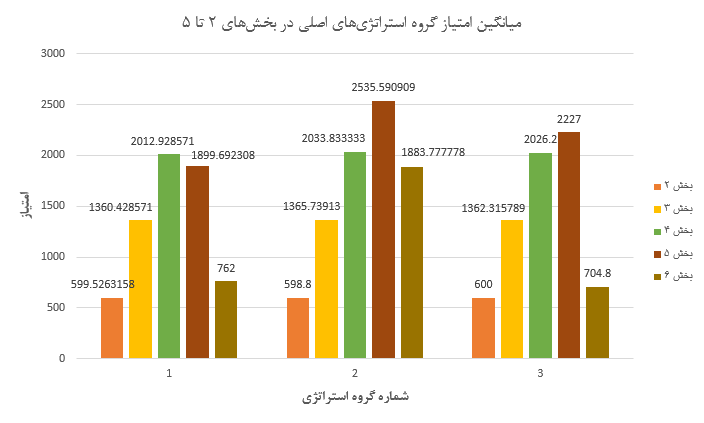
\includegraphics[scale=0.8]{Figures/part2-5AvgScores.png}
\caption{\label{fig:part2to5avgscores}
میانگین امتیاز هر گروه استراتژی در بخش‌های مختلف
}
\end{figure}




\chapter{جمع‌بندی و نکته‌های پایانی}
\label{chapter:conclusion}
\thispagestyle{plain}
در این پژوهش، سعی کردیم تاثیر انواع ویژگی‌های محتوایی را در شناسایی وب‌گاه‌های هرز فارسی بررسی کرده و یک روش با کارایی بالا برای شناسایی این نوع از وب‌گاه‌ها ارائه دهیم. همچنین، با توجه به خصوصیات خاص وب‌گاه‌های هرز، دو روش مبتنی بر پیوند برای رتبه‌بندی وب‌گاه‌ها ارائه دادیم. در نهایت برای بهبود کیفیت رتبه‌بندی، روشی را معرفی کردیم که از ویژگی‌های محتوایی نیز در کنار ویژگی‌های پیوندی استفاده می‌کند. در این فصل، ابتدا مرور مختصری بر دستاوردهای این پژوهش داشته و در ادامه، به منظور بهبود و گسترش این پژوهش، پیشنهادهایی را برای کارهای آینده ارائه می‌دهیم. 



\newpage
\thispagestyle{empty}
\mbox{}

%  : \linespread{1.2}
\linespread{1}


\small{
\bibliographystyle{ieeetr-fa}
\renewcommand{\bibname}{مراجع}
\clearpage
\bibliography{ref}
\addcontentsline{toc}{chapter}{مراجع}
}

\newpage
\thispagestyle{empty}
\mbox{}
\begin{multicols}{2}
\begin{doublespace}

\glossarystyle{mylistLa}
\printglossary[type=latin]
\addcontentsline{toc}{chapter}{واژه‌نامه انگلیسی به فارسی}

\newpage
\thispagestyle{empty}
\mbox{}

\clearpage
\glossarystyle{mylistFa}
\printglossary[type=persian]
\addcontentsline{toc}{chapter}{واژه‌نامه فارسی به انگلیسی}
\end{doublespace}
\end{multicols}

\begin{latin}
\pagestyle{empty}


% LATIN ABSTRACT
\newpage
\thispagestyle{empty}
\mbox{}
\newpage
\vspace*{-2cm}
{\centering\small{\bf{Abstract}} \par \vskip .1cm}
\begin{doublespace} \normalsize

In recent years, due to the increasing amount of data available on the internet, the use of search engines to retrieve relevant information from the World Wide Web has become pervasive. Among the huge number of websites, the ones which succeed to appear more frequently and in higher ranks of search engine results would receive more visitors. So, spammers struggle to achieve a higher than deserved rank for their websites using some illegal techniques called web spamming. 
Although various methods have been used for combatting web spamming, we could basically categorize them into three groups: content-based methods, link-based methods, and the methods based on miscellaneous data. 
In this thesis, we focus on content-based and link-based methods, and also their combination.

Despite the existence of many spam detection methods, the search engines do not perform well in detecting Persian spam websites. Thus, in this thesis, after preparing a corpus of spam and non-spam Persian websites, we analyze the effectiveness of many previously proposed content-based features on detecting Persian spam websites. To improve the performance of classification, we present a number of new content-based features and examine a number of feature selection method. As another approach, we propose a new Persian spam detection system which uses an improved version of bag-of-words model and has better performance in detecting Persian web spam. Due to the prevalence of link-based spamming methods, we analyze some of these methods and propose two new algorithms which do not have the weaknesses of previous methods. In the first algorithm, to improve the process of label propagation, we use three mechanisms: optimized seed selection, edge weighting, and seed expansion. In the second algorithm, we improve the quality of websites ranking, using label propagation in both forward and backward directions. Finally, we propose a combined method, which uses the content-based probability of being spam (non-spam) to propagate the spam (non-spam) score of websites. Using this method, we increase the performance of ranking websites.
 
Finally, to evaluate the proposed methods and compare their performance with the existing methods for this task, we have conducted several experiments on different datasets. Experiment results indicate that the proposed methods have a good performance in detecting web spam.




\end{doublespace}
{\par\vspace{2mm}}
\noindent\textbf{Keywords: }\textit{Spamming, Web Spam, Spam Detection, Label Propagation, Content-Based Features}
% END OF LATIN ABSTRACT

\newpage
\mbox{}


%%%%%%%%%%%%%%%%%%%%%%%%%%%%%
% LATIN TITLE PAGE
%%%%%%%%%%%%%%%%%%%%%%%%%%%%%
\font\titlefont=cmssbx10 scaled 2074
\font\supervisorfont=cmbxti10
\newpage
\thispagestyle{empty}
\begin{center}
\begin{tabular}{lp{7cm}r}

\includegraphics[width=3.8cm]{Figures/eng.png} & & 
\includegraphics[width=2.8cm]{Figures/ut.png} \\
\end{tabular}

\vskip 1cm
\Large{\bfseries
University of Tehran \par
School of Electrical and Computer Engineering}
\large
\par
\vskip 1.5cm
\addtolength{\baselineskip}{5mm}
{\titlefont Detecting Persian Spam Web Pages} \par
\addtolength{\baselineskip}{-5mm}
\vskip 1cm
{\bfseries By}\par
{\Large\bfseries Elahe Rabbani}\par
\vskip 1cm
Supervisors: \\
{\supervisorfont\Large Dr. Azadeh Shakery} \\
%{\supervisorfont\Large Dr. Masoud Asadpour}%
\par
\vskip 2cm
{A thesis submitted to the Graduate Studies Office \\ in partial fulfillment of the requirements \\ for the degree of Master of Science \par
in
\par
\vskip .7cm
\large Computer Engineering}
\par
\vskip .04cm
{September 2014}
\par
\vfill
\end{center}
%%%%%%%%%%%%%%%%%%%%%%%%%%%%%
% END OF LATIN TITLE

\end{latin}
\end{document}‍
